


\tikzset{every picture/.style={line width=0.75pt}} %set default line width to 0.75pt        

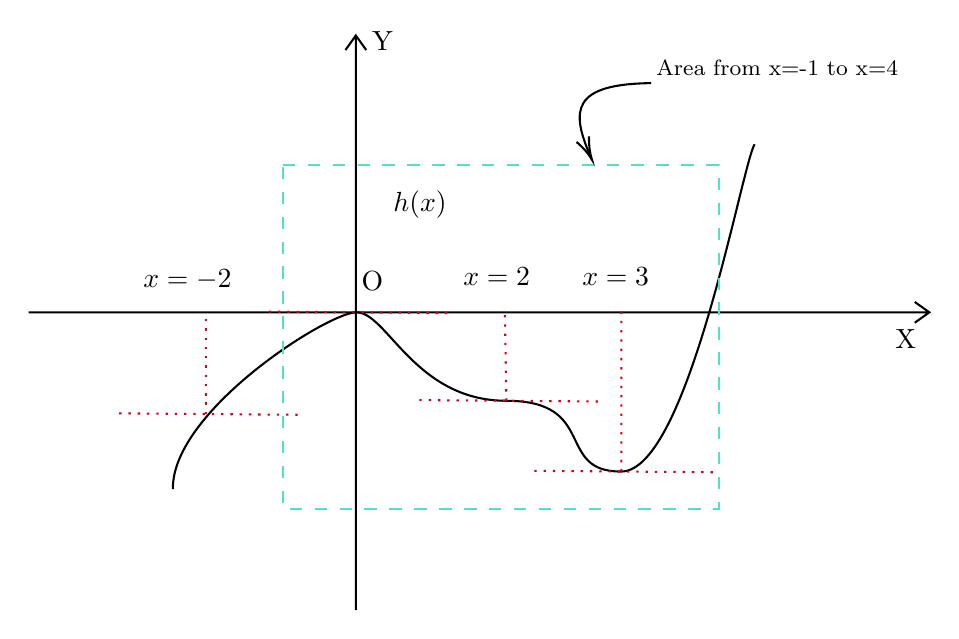
\begin{tikzpicture}[x=0.75pt,y=0.75pt,yscale=-1,xscale=1]
%uncomment if require: \path (0,300); %set diagram left start at 0, and has height of 300

%Shape: Axis 2D [id:dp9944819171450985] 
\draw  (118.09,141.78) -- (552,141.78)(275.7,8.4) -- (275.7,285.24) (545,136.78) -- (552,141.78) -- (545,146.78) (270.7,15.4) -- (275.7,8.4) -- (280.7,15.4)  ;
%Curve Lines [id:da27355266451050975] 
\draw    (187.56,227) .. controls (186.78,190.07) and (260.88,142.49) .. (275.7,141.78) .. controls (290.52,141.07) and (303.78,184.39) .. (348.24,184.39) .. controls (392.7,184.39) and (371.38,218.69) .. (403.62,218.48) .. controls (435.86,218.27) and (461.57,71.44) .. (467.81,60.79) ;
%Straight Lines [id:da590418359643835] 
\draw [color={rgb, 255:red, 208; green, 2; blue, 27 }  ,draw opacity=1 ] [dash pattern={on 0.84pt off 2.51pt}]  (392.31,184.74) -- (304.17,184.03) ;
%Straight Lines [id:da6199838448049988] 
\draw [color={rgb, 255:red, 208; green, 2; blue, 27 }  ,draw opacity=1 ] [dash pattern={on 0.84pt off 2.51pt}]  (447.69,218.83) -- (359.55,218.12) ;
%Straight Lines [id:da4934879921966593] 
\draw [color={rgb, 255:red, 208; green, 2; blue, 27 }  ,draw opacity=1 ] [dash pattern={on 0.84pt off 2.51pt}]  (319.77,142.13) -- (231.63,141.42) ;
%Straight Lines [id:da04786413405641343] 
\draw [color={rgb, 255:red, 208; green, 2; blue, 27 }  ,draw opacity=1 ] [dash pattern={on 0.84pt off 2.51pt}]  (348.24,184.39) -- (347.5,141.99) ;
%Straight Lines [id:da1730175943856178] 
\draw [color={rgb, 255:red, 208; green, 2; blue, 27 }  ,draw opacity=1 ] [dash pattern={on 0.84pt off 2.51pt}]  (403.62,218.48) -- (403.66,141.46) ;
%Straight Lines [id:da6218480984588155] 
\draw [color={rgb, 255:red, 208; green, 2; blue, 27 }  ,draw opacity=1 ] [dash pattern={on 0.84pt off 2.51pt}]  (203.59,190.78) -- (203.59,142.52) ;
%Straight Lines [id:da684943730116574] 
\draw [color={rgb, 255:red, 208; green, 2; blue, 27 }  ,draw opacity=1 ] [dash pattern={on 0.84pt off 2.51pt}]  (247.66,191.14) -- (159.52,190.43) ;
%Shape: Rectangle [id:dp12176029931702059] 
\draw  [color={rgb, 255:red, 80; green, 227; blue, 194 }  ,draw opacity=1 ][dash pattern={on 4.5pt off 4.5pt}] (240.5,71) -- (450.5,71) -- (450.5,236.34) -- (240.5,236.34) -- cycle ;
%Curve Lines [id:da991809814222433] 
\draw    (418,31.34) .. controls (379.98,31.83) and (379.02,44.2) .. (388.73,66.6) ;
\draw [shift={(389.5,68.34)}, rotate = 245.92] [color={rgb, 255:red, 0; green, 0; blue, 0 }  ][line width=0.75]    (10.93,-3.29) .. controls (6.95,-1.4) and (3.31,-0.3) .. (0,0) .. controls (3.31,0.3) and (6.95,1.4) .. (10.93,3.29)   ;

% Text Node
\draw (276.96,120.71) node [anchor=north west][inner sep=0.75pt]   [align=left] {O};
% Text Node
\draw (292.28,81.7) node [anchor=north west][inner sep=0.75pt]    {$h( x)$};
% Text Node
\draw (534.19,148.41) node [anchor=north west][inner sep=0.75pt]   [align=left] {X};
% Text Node
\draw (282.06,5.13) node [anchor=north west][inner sep=0.75pt]   [align=left] {Y};
% Text Node
\draw (325.97,118.98) node [anchor=north west][inner sep=0.75pt]    {$x=2$};
% Text Node
\draw (383.3,118.98) node [anchor=north west][inner sep=0.75pt]    {$x=3$};
% Text Node
\draw (171.8,119.52) node [anchor=north west][inner sep=0.75pt]    {$x=-2$};
% Text Node
\draw (419,19) node [anchor=north west][inner sep=0.75pt]   [align=left] {{\footnotesize Area from x=-1 to x=4 }};


\end{tikzpicture}